\documentclass[leqno]{article}

\usepackage{array}
\usepackage{fancyvrb}
\usepackage{multicol}
\usepackage{centernot}

\usepackage[utf8]{inputenc}
\usepackage{mathtools}
\usepackage{amsmath}
\usepackage{amssymb}
\usepackage{amsmath,amsfonts,amssymb,amsthm,epsfig,epstopdf,titling,url,array}
\usepackage{hyperref}
\usepackage{tikz}
\usepackage{graphicx}
\usepackage{multicol}

\usepackage{import}
\usepackage{xifthen}
\usepackage{pdfpages}
\usepackage{transparent}
\usepackage{wrapfig}

\newcommand{\incfig}[1]{%
  \def\svgwidth{0.9\columnwidth}
  \import{./figures/}{#1.pdf_tex}
}

\newcommand{\norm}[1]{\lvert \lvert #1 \rvert \rvert }
\newcommand{\cond}[1]{\text{cond(} #1 \text{)}}
\renewcommand{\th}{\textbf{Th:} \ }
\newcommand{\h}{\hspace{1em}}
\newcommand{\R}{\mathcal{R}}

\renewcommand{\phi}{\varphi}

\newcommand{\T}{\mathcal{T}}
\newcommand{\A}{\mathcal{A}}
\renewcommand{\S}{\mathcal{S}}

\newcommand{\st}{\ | \ }
\newcommand{\K}{\mathbb{K}}
\renewcommand{\P}{\mathbb{P}}
\newcommand{\Rcal}{\mathcal{R}}
\renewcommand{\A}{\mathcal{A}}
\newcommand{\B}{\mathbb{B}}

\title{Álgebra Multilineal}

\begin{document}
\maketitle
\tableofcontents
\newpage

\section{Formas de Jordan}
Por el \textit{Primer teorema de Descomposición} tenemos que todo espacio se puede escribir como suma directa de núcleos de potencias de $f-\lambda_iI$, donde $\lambda_i$ son los VAPs del endomorfismo $f$:
$$
E = \ker(f-\lambda_1I)^m_1 \oplus \cdots \oplus \ker(f-\lambda_rI)^{m_r}
$$
Además, se cumple
$$
0 = \ker(f-\lambda_iI)^0\subset \ker(f-\lambda_iI)^1 \subset \cdots \subset \ker(f-\lambda_iI)^{m_i}=\cdots
$$
Es por esto por lo que todo endomorfismo se puede descomponer en endomorfismos más simples, ya que los VAPs generan subespacios invariante. Por ello trabajaremos con endomorfismos de un solo VAP (con multiplicidad $>1$) \\
\\
Para todo el capítulo definimos:
\begin{itemize}
    \item $f:E\to E,\ n = \dim (E)$
    \item $Q_f(t) = (\lambda - t)^n,\ m_f(t) = (t-\lambda)^m$
    \item $N^i = \ker(f-\lambda I)^i = \ker(g^i),\ d_i = \dim(N^i)$
\end{itemize}
Para hacerlo más visual desarrollaremos el concepto de \textit{Edificio de Jordan}. Calcularemos los subespacios $N^i$ y construiremos el edificio tal que el el $i-$ésimo piso haya vectores de $N^i$, pero no de $N^{i-1}$ y además sean l.i. entre sí. Buscaremos también que $g(u_{i,j})=u_{i-1, j}$, es decir, que para bajar un piso (en la misma columna) solo se deba aplicar $g$. Esto es lo que dará la forma a la matriz de Jordan.

\begin{multicols}{2}

 \text{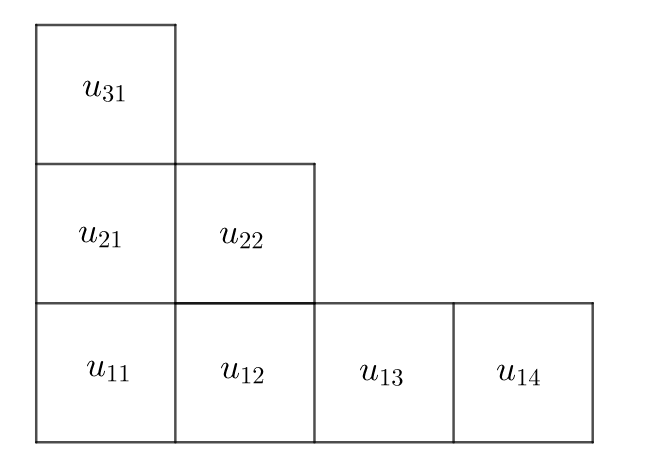
\includegraphics[scale=0.3]{Jordan.png} } 
\columnbreak 
$$ 
\implies \qquad 
\begin{pmatrix}
\lambda & & & & & & \\
1& \lambda & & & & & \\
& 1&\lambda  & & & & \\
& & &\lambda  & & & \\
& & &1 &\lambda  & & \\
& & & & &\lambda  & \\
& & & & & &\lambda 
\end{pmatrix}
$$

\end{multicols}

\textbf{Proposición}: Son equivalentes
\begin{itemize}
    \item $u_1, \ldots , u_s$ l.i. de $N^i$,\  $[u_1, \ldots , u_s]\cap N^{i-1}=0$
    \item $\dim([u_1, \ldots, u_s]) = s, \ [u_1, \ldots , u_s]\oplus N^{i-1} \subseteq N^i$
    \item $g(u_1), \ldots , g(u_s)$ l.i. de $N^{i-1}$,\  $[g(u_1), \ldots , g(u_s)]\cap N^{i-2}=0$
    \item $\dim([g(u_1), \ldots, g(u_s)]) = s, \ [g(u_1), \ldots , g(u_s)]\oplus N^{i-2} \subseteq N^{i-1}$
    \item $g^{i-1}(u_1), \ldots g^{i-1}(u_s)$ l.i. de $N^1$
\end{itemize}

\section{Formas cuadráticas}
\subsection{Definiciones}
Para esta sección $\varphi:E\to E$ será una forma bilineal simétrica y $\dim(E)=n$ \\
\\
Una forma cuadrática es una aplicación $q:E\to \mathbb{K}$ tal que existe $\varphi$ que cumple $q(x)=\phi(x,x)$. Existe una biyección entre las formas cuadráticas y formas bilineales simétricas:
$$
q(x) = \phi(x,x) \qquad \varphi(x,y)=\frac{1}{2}(q(x+y)-q(x) - q(y))
$$



La matriz $M_e(q)$ cumple $q(x)= x^TM_ex$ donde $x$ está escrito en base $e$. Por el \textit{Teorema Espectral}, como $M$ es simétrica, podemos diagonalizarla en una base ortogonal. Podemos usar la diagonalización o el Método de Gauss. \\
\\
\subsection{Rango, Radical e Indice}
Nos encontramos con tres propiedades de las formas cuadráticas:
\begin{itemize}
    \item \textbf{Rango} $rang(\phi) = rang(M(\phi))$
    \item \textbf{Radical} $rad(\phi)=\{x\in E \ | \ \phi(x,y)=0 \forall y\in E\}$
    \item \textbf{Indice} $\begin{cases} 
    i_+(\phi) &= \# \lambda_i>0 \\
    i_-(\phi) &= \# \lambda_i<0 \\
    i(\phi) &= \min(i_+, i_-)
    \end{cases}$
\end{itemize}

\subsection{Clasificación Afín y Proyectiva}
\textbf{Afín}\\
$\phi:E\to E$ es \textit{Afín-equivalente} a $\psi:F\to F$ (\textbf{rellenar}) si existe un isomorfismo $\alpha:E\to F$ tal que $\psi = \phi\circ(\alpha^-1\times \alpha^-1)$ \\
\\
Si $\mathbb{K} = \mathbb{R} \implies rang(\phi) = rang(\psi), \ i_+(\phi) = i_+(\psi)$ \\
\\
\textbf{Proyectiva}\\
$\phi:E\to E$ es \textit{Proyectivo-equivalente} a $\psi:F\to F$ (\textbf{rellenar}) si existe un isomorfismo $\alpha:E\to F$ y un $\lambda\in \mathbb{K}-\{0\}$ tal que $\psi = \lambda\phi\circ(\alpha^-1\times \alpha^-1)$ \\
Si $\mathbb{K} = \mathbb{R} \implies rang(\phi) = rang(\psi), \ i(\phi)  i(\psi)$


\section{Tensores}
Un \textit{p-q tensor} es un elemento $f$ del espacio vectorial definido como
$$
\boxed{\T_p^q(E)=\{ f: E^{\times p}\times (E^*)^{\times q} \to \mathbb{K} \st f \text{ multilineal}\} = \mathcal{L}(E^{p)}, (E^*)^{q)};\mathcal{K})}
$$
Los tensores \textit{Covariantes} son los que pertenecen a $\T_p:=\T_p^0$ \\
Los tensores \textit{Contravariantes} son los que pertenecen a $\T^q:=\T_0^q$ \\
\\
Podemos escribir la base de un tensor $f\in \T_p^q$ como
$$
\mathcal{B}_p^q=\{e^{i_1}\otimes \ldots \otimes e^{i_p}\otimes e_{j_1}\otimes \ldots \otimes e_{j_q} \st i_k, j_k\in [n]\} = \{e^{\otimes I}\otimes e_{\otimes J}\}
$$
Observamos que la dimensión de $f$ es $n^{(p+q)}$\\
\\
Si queremos expresar un tensor $f$ en la base $\mathcal{B}$ sus componentes son:
\[
  f= \sum f(e_{\times I}e^{\times J})(e^{\otimes I}e_{\otimes J})
\] 

\subsection{Producto tensorial}
Definimos el producto tensorial como
$$
f\otimes g:E^{\times(p+r)}\times (E^*)^{\times(q+s)} \to \mathbb{K} \text{ cumpliendo } \boxed{f\otimes g (x, y, u, v) = f(x, u)g(y,v)  }  
$$

\subsection{Cambio de base}
El producto tensorial entre dos matrices (o producto de Kronecker) se define como
$$
M\otimes N = \begin{pmatrix}
m_{1,1}N & \cdots & m_{1,r}N\\
\vdots &  & \vdots \\
m_{r,1}N & \cdots & m_{r,r}N
\end{pmatrix}
$$

Sea $M_{u, e} = \begin{pmatrix}
u_1(e^1) & u_2(e^1) \\
u_1(e^2) & u_2(e^1)
\end{pmatrix}$ y $M_{u^*, e^*} = \begin{pmatrix}
u^1(e_1) & u^2(e_1) \\
u^1(e_2) & u^2(e_1)
\end{pmatrix}$ las matrices de cambio de base.\\
Una propiedad importante es que $M_{u, e}^TM_{u^*, e^*} = I$.
\\
Si ahora queremos calcular el cambio de base de $u^*\otimes u$ a $e^*\otimes e$ tenemos que
$$
M_{u^*\otimes u, e^*\otimes e} = M_{u^*, e^*}\otimes M_{u,e}
$$

\subsection{Tensores simétricos y antisimétricos}
$f\in\T_p(E)$ es \textit{Simétrico} ($f\in \S$) si $f(x_1, \ldots, x_i, \ldots, x_j, \ldots, x_p) = f(x_1, \ldots, x_j, \ldots, x_i, \ldots, x_p)$ \\
$f\in\T_p(E)$ es \textit{Antisimétrico} ($f\in \A$) si $f(x_1, \ldots, x_i, \ldots, x_j, \ldots, x_p) = -f(x_1, \ldots, x_j, \ldots, x_i, \ldots, x_p)$ \\
\\
Podemos construir dos operadores: el de simetrización y el de antisimetrización
$$
\S(f) = \frac{1}{p!} \sum_{\sigma \in \frak{S}_n} \sigma f, \qquad \A(f) = \frac{1}{p!} \sum_{\sigma \in \frak{S}_n} \epsilon(\sigma)\sigma f
$$

Propiedades de estos operadores
\begin{itemize}
    \item $\S(f)\in \S_p(E)$ y $\A(f)\in \A_p(E)$
    \item $\S, \A$ son proyectores $\S^2=\S,  \A^2=\A$
    \item $\T_p(E)=\S_p(E)\oplus \ker(\S) = \A_p(E)\oplus \ker(\A)$
\end{itemize}

\subsection{Producto exterior}
Sean $f\in\T_p(E), g\in \T_q(E) $ definimos el producto exterior como
$$
f\wedge g := \frac{(p+q)!}{p!q!}\A(f\otimes g) = \frac{1}{p!q!}\sum_\sigma \epsilon(\sigma)(f\otimes g) \in \A_{p+q}(E)
$$
Algunas propiedades básicas son
\begin{itemize}
    \item $(f\wedge g)\wedge h=f\wedge(g\wedge h)$
    \item $(\lambda f)\wedge(f\wedge g) = f\wedge(\lambda g)$
    \item $f\wedge(g+g') = (f\wedge g) + (f\wedge g')$
    \item $g\wedge f = (-1)^{pq} f\wedge g$
\end{itemize}
Podemos construir la siguiente base de el espacio de tensores antisimétricos $\A_p(E)$
$$
\mathcal{B} = \{ e^I \st I\in \mathcal{L}_p \}, \text{ donde } \mathcal{L}_p = \{ (i_1, \dots, i_p) \st 1\leq i_1 < \ldots <i_p\leq n \}
$$

\subsection{Propiedades}
\begin{itemize}
    \item $f=\sum f(e_{\times I}, e^{\times J})e^{\otimes I}e_{\otimes J}$
    \item $\sigma (u^1\otimes \ldots \otimes u^p) = u^{\tau(1)}\otimes \ldots \otimes u^{\tau(p)}, \quad (\tau := \sigma^{-1})$
    \item $\A(\A(f)\otimes g) = \A(f\otimes\A(g)) = \A(f\otimes g)$
    \item $u^1\wedge \ldots \wedge u^p = p!\A(u^1\otimes \ldots \otimes u^p) = \sum_\sigma \epsilon(\sigma)u^{\sigma(1)}\otimes \ldots \otimes u^{\sigma(p)}$
    \item $\sigma(u^1\wedge \ldots \wedge u^p) = \epsilon(\sigma)u^1\wedge \ldots \wedge u^p$
    \item $(u^1\wedge \ldots \wedge u^p)(x_1, \ldots, x_p) = \det (u^i(x_j))$
    \item $e^{\wedge I}(e_{\times J}) = \delta_I^J$
\end{itemize}




\section{Espacio proyectivo}
\subsection{Definiciones}
Un espacio proyectivo sobre el cuerpo $\K$ es una terna $(\P, E, \pi)$ siendo $\pi:E-{0}\to \P$ una aplicación exhaustiva que satisface $\pi(x)=\pi(y)\iff x=\lambda y$.\\
Denotaremos $p = \pi(x) = [x]$. Definimos $\dim\P = \dim E -1$. \\
\\

\begin{multicols}{2}[\columnsep2em] 
Un Espacio proyectivo se puede pensar como la unión disjunta de un $\K$ espacio vectorial de la misma dimensión y un espacio proyectivo de una dimensión menos:
$$
\P^n = \K^n \sqcup \P^{n-1}
$$
\columnbreak


    \incfig{ProyectivoVisual}

\end{multicols}



%Un Espacio proyectivo se puede pensar como la unión disjunta de un $\K$ espacio vectorial de la misma dimensión y un espacio proyectivo de una dimensión menos:
%$$
%\P^n = \K^n\amalg P^{n-1}
%$$



\subsection{Variedades lineales proyectivas}
Una variedad lineal proyectiva (vlp) $L = [F]$definida por el subespacio $F$ es el subconjunto de $\P$ definido como $\pi(F-{0})$. \\
Propiedades:
\begin{itemize}
 \item $\dim L = \dim F - 1$
 \item $L_1 \subseteq L_2 \iff F_1\subseteq F_2$
 \item Si $L_1\subseteq L_2 \implies \dim L_1 \leq \dim L_2$
 \item Si $L_1 \subseteq L_2 $ y $\dim L_1 = \dim L_2 \implies L_1 = L_2$
\end{itemize}
En cuanto a la intersección y el joint ($\vee$), sean $L_1 = [F_1], L_2 = [F_2]$:
\begin{itemize}
 \item $L_1\cap L_2 = [F_1\cap F_2]$
 \item $L_1\vee L_2 = [F_1 + F_2]$
 \item Grassmann: $ \dim L_1 + \dim L_2 = \dim L_1\cap L_2 + \dim L_1\vee L_2$
\end{itemize}

\subsection{Referencias proyectivas}
Una referencia proyectiva es un conjunto $\Rcal = \{p_0, \ldots, p_n; U\}$ de $n+1$ puntos ordenados li y un punto unidad $U$ combinación lineal de todos los otros con ningún coeficiente 0. \\
\\
Cuando $U = [e_0 + \ldots + e_n]$ con $p_i = [e_i]$, entonces la referencia se denomina "adaptada". Este punto fuerza a que el factor de proporcionalidad sea constante, y por tanto, que las coordenadas estén bien definidas.

\subsection{Cambio de base}
Sean $\Rcal_1 = \{p_0, \ldots, p_n; U\}$, $\Rcal_2 = \{q_0, \ldots, q_n; V\}$ dos referencias proyectivas de $\P$. Sean $e_0, \ldots, e_n$ y $u_0, \ldots;u_n$ bases adaptadas. Sea $M_{u,e}$ la matriz de cambio de base. \\
\\
La matriz de cambio de referencia de $\Rcal_2\to \Rcal_1$ es $[M_{u, e}]\in \P(M_{n+1}(\mathbb{K}))$\\
\\
Sean $x = x_0e_0 + \ldots + x_ne_n, y = y_0u_0 + \ldots + y_nu_n$. Podemos expresar sus coordenadas proyectivas como:
$$
X = \begin{pmatrix} x_0 \\ \vdots \\ x_n \end{pmatrix} = (x_0:\ldots:x_n) , \qquad Y = \begin{pmatrix} y_0 \\ \vdots \\ y_n \end{pmatrix} = (y_0:\ldots:y_n), \qquad X = M_{u, e}Y
$$

(Completar)

\subsection{Coordenada Absoluta y razón doble}
Sea $q = [xe_0 + ye_1]$. Definimos la \textit{coordenada absoluta} $\theta(q) = \frac{x}{y}$ si $q\neq p_0$ y $\theta(p_1) = \infty$. Esta aplicación $\theta :\P^1 \to \Bar{\K}$ está bien definida. \\
\\
Definimos ahora la \textit{razón doble} de $q_1, q_2, q_3, q_4$:
$$
(q_1, q_2, q_3, q_4) = \frac{\det(v_1, v_3) \det(v_2, v_4)}{\det(v_1, v_4) \det(v_2, v_3)} = \frac{(\theta_3 - \theta_1)(\theta_4-\theta_2)}{(\theta_4 - \theta_1)(\theta_3 - \theta_2)}
$$
La razón doble de cuatro puntos no depende de la referencia. \\
Si $\Rcal=\{p_1, p_2;U\}$, algunas propiedades:
\begin{itemize}
 \item $(q_1, q_2, q_3, q_4)(q_1, q_2, q_4, q_5) = (q_1, q_2, q_3, q_5)$
 \item $(q_1, q_2, q_3, q_4) = 0 \iff q_1 = q_3$ ó $q_2 = q_4$
 \item $(q_1, q_2, q_3, q_4) = \infty \iff q_2 = q_3$ ó $q_1 = q_4$
 \item $(q_1, q_2, q_3, q_4) = 1 \iff q_1 = q_2$ ó $q_3 = q_4$
 \item $(p_1, p_2, q_3, q_4)=\frac{\theta(q_4)}{\theta(q_3)}$  
 \item $(p_1, p_2, U, q_4)=\theta(q_4)$
\end{itemize}


\subsection{Teoremas}
\subsubsection{Teorema de Desargues}
\subsubsection{Teorema de Pappus}
 

\section{Espacio proyectivo y afín}
\subsection{Clausura proyectiva}
Recordemos que un \textit{espacio afín} es una terna $(\A, E, s)$, que satisface:
\begin{itemize}
  \item $\exists \ s:\A \times E\to \A$ tal que $s(a, u) = a+u$
  \item $(a+u) + v = a + (u + v)$
  \item Para cada $a, b \in \A \ \exists ! \ u\in E $ tal que $a+ u = b$
\end{itemize}
La \textit{clausura proyectiva} de un espacio afín es un espacio proyectivo $\bar{\A}$ tal que $\A \cong \bar{\A}-\A_\infty$, donde $\A_\infty$ es el hiperplano del infinito. \\
\\
(Dibujo fancy)\\
\\
Podemos construir una aplicación $i: \A \to \P$ ... \\
\\
Sea $\B = \P-H$. Sea $L = [F]$ vlp no contenida en $H$. Si $q\in L\cap \B \implies L\cap B$  

\subsection{Coordenadas}

\subsection{Pasar de coordenadas afines a proyectivas}
\underline{Ejemplo 1} \\
\[
  L = \begin{pmatrix} 2 \\ 0\\0\\1 \end{pmatrix} + [\begin{pmatrix} 1\\0\\0\\1 \end{pmatrix} ] \implies \left(\begin{array}{@{}c|c@{}} 1 & x_1-2 \\ 0 & x_2 \\ 0 & x_3 \\ 1 & x_4-1 \end{array}  \right) \sim \left(\begin{array}{@{}c|c@{}} 1 & x_1-2 \\ 0 & x_2 \\ 0 & x_3 \\ 0 & x_4-x_1+1 \end{array} \right) \implies
  \begin{cases}
    x_2 = 0 \\
	x_3 = 0 \\
	x_4-x_1+1 = 0
  \end{cases}
\] 
Para calcular $\overline{L}$ podemos (1) hacer el join de los puntos de la clausura (los puntos afines serán puntos con cordenada $x_0=1$ y los vectores puntos con coordenada $x_0=0$) o (2) homogeneizar las ecuaciones implícitas:
 \[
   (1): \overline{L} = (1:2:0:0:1)\vee (0:1:0:0:1) \qquad (2): \overline{L}:\begin{cases}
     x_2=0\\
	 x_3=0\\
	 x_4-x_1+x_0=0
   \end{cases}
\] 

\section{Dualidad}
El espacio dual de $\P$ es el conjunto $\P^* = \{H | H \text{ hiperplano de }\P\}$ \\
Se comprueba que $\P^*$ es también un espacio proyectivo $(\P^*, E^*, \pi^*)$
Podemos definir naturalmente el dual de una vlp como:
$$
L = [F]_\pi \implies L^* = [F^\perp]_{\pi^*}
$$

Existe una biyección $Vlp_d(\P) \iff Vlp_{n-d-1}(\P^*)$ \\
\\

Propiedades:
\begin{itemize}
  \item $[\omega]_{\pi^*} := [\ker(\omega)]_\pi$
  \item $L_1\subset L_2 \implies L_2^*\subset L_1^*$
  \item $L = L_1\cap L_2 \implies L^* = L_1^* \vee L_2^*$
  \item $L = L_1\vee L_2 \implies L^* = L_1^* \cap L_2^*$

\end{itemize}

\subsection{Principio de dualidad}
Una frase es dualizable y solo si es composición de dimensiones, inclusiones, contenciones, intensecciones y joins de vlps:
\begin{itemize}
  \item $\mathcal{F}_1: \dim L = d \implies \mathcal{F}_1^*: dim L = n-d-1$
  \item $\mathcal{F}_2: L_1 \supset L_2 \implies \mathcal{F}_2^*: L_1 \subset L_2$
  \item $\mathcal{F}_3: L_1 \subset L_2 \implies \mathcal{F}_3^*: L_1 \supset L_2$
  \item $\mathcal{F}_4: L = L_1 \cap L_2 \implies \mathcal{F}_4^*: L_1 \vee L_2$
  \item $\mathcal{F}_5: L = L_1 \vee L_2 \implies \mathcal{F}_5^*: L_1 \cap L_2$
\end{itemize}
Denotamos como \textit{enunciado} $\mathcal{E}$, una hipótesis $\mathcal{H}$ que implica una tesis $\mathcal{T}$: $\mathcal{E}: \mathcal{H}\to \mathcal{T}$.\\
El \textit{Principio de dualidad} nos dice que si  $\mathcal{E}: \mathcal{H}\to \mathcal{T}$, entonces se cumple también $\mathcal{E}^*: \mathcal{H}^*\to \mathcal{T}^*$ \\
\\
Con este principio podemos dualizar los teoremas proyectivos que ya conocemos como Desargues o Pappus. En el caso de Desargues llegamos a su recíproco, y en el de Pappus a un nuevo resultado.




\section{Proyectividades}

\subsection{Proyectividades}
Una proyectividad es una aplicación $f:\P \to \P'$ inducida por un isomorfismo  $\varphi:E\to E'$ tal que  $f=[\varphi]$. En particular una homografía es una proyectividad $f:\P\to \P$

\subsection{Propiedades}
Propiedades de las vlp:
\begin{itemize}
    \item Si $L = [F] \implies f(L) =  [\phi(F)]$ y $\dim f(F) = \dim L$
    \item $f|_L: L\to f(L)$ definida por $f|_L = [\phi|_F]$
    \item $L_1\subseteq L_2 \iff f(L_1) \subseteq f(L_2)$
    \item $f(L_1\cap L_2) = f(L_1)\cap f(L_2)$
    \item $f(L_1\vee L_2) = f(L_1)\vee f(L_2)$
    \item $f(q_0\vee \ldots \vee q_m) = f(q_0)\vee \ldots \vee f(q_m)$
    \item $q_0, \ldots, q_m$ l.i. $\implies f(q_0), \ldots, f(q_m)$ l.i.
\end{itemize}
Propiedades de las referencias:
\begin{itemize}
    \item Si $\R = \{p_0, \ldots, p_n; U\} \implies f(\R)=\{f(p_0), \ldots, f(p_n); U\}$ es referencia
	\item Si $e$ es base adaptada a $\mathcal{R} \implies \phi(e)$ base adaptada a $f(\mathcal{R})$ 
	\item $q_1, q_2, q_3, q_4$ alineados en $\P \implies$ $f(q_1), f(q_2), f(q_3), f(q_4)$ alineados y $(q_1, q_2, q_3, q_4) = (f(q_1), f(q_2), f(q_3), f(q_4))$
	\item La proyectividad queda determinada por la imagen de la base.
\end{itemize}

\subsection{Caracterización geométrica de las proyectividades}
Si $\dim\P\ge 1$ tenemos la caracterización:
\[
  f \text{ proyectividad } \iff \begin{cases}
  f \text{ biyectiva} \\
  f \text{ colineación} \\
  f \text{ conserva razón doble}
\end{cases}
\]
Para $\dim \P = 1$ lo mismo sin colineación.

\subsection{Tipos de proyectividades}
\subsubsection{Perspectividad}
\begin{minipage}{0.7\textwidth}
Dadas  $V_1, V_2$ vlp disjuntas de dimensión $d$.  $W$ la vlp complementaria a ambas con dimensión  $n-d-1$.\\
La pespectividad de centro $W$ sobre  $V_1, V_2$ es:
\begin{align*}
  f: V_1 & \to V_2  \\
  p & \to f(p))(W\lor p)\cap V_2
\end{align*}
\end{minipage}  
\begin{minipage}{0.3\textwidth}
  \incfig{Perspectividad}
\end{minipage}
Por el \textbf{Teorema de Poncelet} la proyectividad $f: V_1\to V_2$ es composición de perspectividades.

\subsubsection{Homologías}
\begin{minipage}{0.7\textwidth}
Una \textbf{Homologías} de eje $H$ hiperplano es una homografía  $f$ que deja fijo  $H$ y tiene un único punto fijo $p_H$. Además toda recta por $p_H$ es invariante.
	 \begin{itemize}
	  \item $p_H\notin H \implies$ homología general. $m_\varphi(t) = (t-a)(t-b)$
	  \item $p_H\in H \implies$ homología especial. $m_\varphi (t) = (t-a)^2$
	\end{itemize}
\end{minipage}
\begin{minipage}{0.3\textwidth}
  \incfig{HomologiaGeneral} 
\end{minipage}

\subsubsection{Involución}
$f$ homografía tal que  $f^2 = I$ con  $f\neq  I$\\
\\
Tenemos que $m_\varphi(t) = t^2-\lambda$: \\
\underline{Caso $\lambda>0$} $\implies A = \begin{pmatrix} \sqrt{\lambda} & & \\ &  \ddots & \\ & & -\sqrt{\lambda}  \end{pmatrix} $  \\
\underline{Caso $\lambda<0$} $\implies \varphi $ no diagonaliza  


\subsection{Matriz de una Proyectividad}
Tenemos que $M_{\mathcal{R}, \mathcal{R}'} = [M_{u, v}(\varphi )]$ donde $[M] = [\lambda M]\ \forall \lambda\ \neq 0$ \\
\\
Propiedades
\begin{itemize}
  \item $M_{\mathcal{R}, \mathcal{R}''}(g\circ f)=M_{\mathcal{R}', \mathcal{R}''}(g)M_{\mathcal{R}, \mathcal{R}'}(f)$
  \item $M_{\mathcal{R}', \mathcal{R}}(f^{-1}) = M_{\mathcal{R}, \mathcal{R}'}(f)^{-1}$ 
  \item $M_{\mathcal{S}, \mathcal{S}'}(f) = M_{\mathcal{R}', \mathcal{S}'}M_{\mathcal{R}, \mathcal{R}'}(f) M_{\mathcal{S}, \mathcal{R}}$
  \item $M_{\mathcal{R}^*}(f^*) = M_{\mathcal{R}}(f)^{T}$ 
\end{itemize}

\subsection{Clasificación de proyectividades}
Clasificaremos las proyectividades respecto a su forma de Jordan como relación de equivalencia. $f\sim g \iff$
el edificio de Jordan es el mismo. \\
\\
Se demuestra que si $L = [F]$ es $f$-invariante $\implies$ $[\rho^{-1}(F^\perp)]$ es invariante.\\
\\

Toda homografía es composición de homologías.

\subsubsection{Puntos fijos y variedades invariantes}
$p$ es un \textbf{punto fijo} de  $f$ $\iff f(p)=p$\\
Los puntos fijos son la clase de los VEPs de $\varphi $, y las variedades fijas la clase espacio generado por los VEPs de mismo VAP de $\varphi $ \\
\\
$V$ es una \textbf{variedad invariante} por  $f \iff f(V) = V$\\
Las variedades invariantes son la clase de los subespacios invariantes de $\varphi $ \\
\\
Propiedades:
\begin{itemize}
  \item $V_1, V_2$ invariantes $\implies$ $V_1\lor V_2, V_1\cap V_2$ invariantes
  \item $p_1, p_2$ puntos fijos $\implies p_1\lor p_2$ recta invariante 
  \item $V$ $f-$invariante  $\implies$ $V^* f^*-$invariante
\end{itemize}

\subsubsection{Homografías en la recta $\mathbb{P}^1$}
El tipo representa las afinidades de las que viene tomando $p_\infty$ como el punto del infinito.
\begin{center}
  \begin{tabular}{|c|c|c|c|c|}
	\hline
    Tipo & Forma de Jordan $\varphi $ & Forma de Jordan $f$ & Puntos Fijos & Vlp invariantes \\
	\hline
	Identidad  & $\begin{pmatrix} a & 0 \\ 0 & a \end{pmatrix} $ & $\begin{pmatrix} 1 & 0 \\ 0 & 1 \end{pmatrix} $ & Todos & Todas \\
	\hline
	Homología general & $\begin{pmatrix} a & 0 \\ 0 & b \end{pmatrix} $ & $\begin{pmatrix} 1 & 0 \\ 0 & \beta \end{pmatrix} $ & $p_0, p_1$ & (por determinar) \\
	\hline
	Homología especial & $\begin{pmatrix} \lambda & 0 \\ 1 & \lambda \end{pmatrix} $ & $\begin{pmatrix} 1 & 0 \\ 1 & 1 \end{pmatrix} $ & $p_1$ & \\
	\hline
	Nada & $\varphi$ no descomponible & $\varphi $ no descomponible & $\emptyset$ & (por determinar) \\
	\hline
  \end{tabular}
\end{center}

\subsubsection{Homografías en el plano $\mathbb{P}^2$}

\begin{center}
\begin{tabular}{|c|c|c|c|c|}
\hline
Tipo & Forma de Jordan $\varphi $ & Forma de Jordan $f$ & Puntos Fijos & Vlp invariantes \\
\hline
Identidad & $\begin{pmatrix} 1 & & \\ & 1 & \\ & & 1 \end{pmatrix}$ & $\begin{pmatrix} 1 & & \\ & 1 & \\ & & 1 \end{pmatrix} $ & Todos & Todas \\
	 \hline
Homología general	 & $\begin{pmatrix} a & & \\ & b & \\  & & b \end{pmatrix} $ & $\begin{pmatrix} a & & \\ & 1 & \\  & & 1 \end{pmatrix} $ & $p_0, L = p_1\lor p_2$ & $p_0^*$ \\
	 \hline
Homología especial	 & $\begin{pmatrix} a & & \\ 1 & a & \\  & & a \end{pmatrix} $ & $\begin{pmatrix} 1 & & \\ 1 & 1 & \\  & & 1 \end{pmatrix} $ & $L = p_1\lor p_2$ & \\
\hline
					 & $\begin{pmatrix} a & & \\ 1 & a& \\  & & b \end{pmatrix} $ & $\begin{pmatrix} 1 & & \\ 1 & 1 & \\  & & a \end{pmatrix} $ & $p_1, p_2$ & $p_1\lor p_2, p_0\lor p_1$   \\
\hline
					 &  $\begin{pmatrix} a & & \\  & b & \\  & & c \end{pmatrix} $ & $\begin{pmatrix} 1 & & \\  & a & \\  & & b \end{pmatrix} $ & $p_0, p_1, p_2$ & $p_0\lor p_1, p_1\lor p_2, p_2\lor p_0$ \\
   \hline
					 & $\begin{pmatrix} a & & \\ 1 & a & \\  & 1 & a \end{pmatrix} $ & $\begin{pmatrix} 1 & & \\ 1 & 1 & \\  & 1 & 1 \end{pmatrix} $ & $p_2$ & $p_1\lor p_2$ \\
\hline
					 & $\begin{pmatrix} a & & \\  & b & c\\  & d & e \end{pmatrix} $ & $\begin{pmatrix} 1 & & \\  & a & b\\  & c & d \end{pmatrix} $  & $p_0$ & $p_1\lor p_2$  \\
					 \hline
\end{tabular}
\end{center}





\section{Cuádricas}
\subsection{Definiciones y propiedades básicas}
Una \textbf{Cuádrica} es el conjunto de puntos $p$ tal que la forma cuadrática $Q(p)=0 \iff x^TAx = 0$\\
\\
$p$ es un  \textbf{Punto singular} de Q $\iff u\in rad(\varphi ) = \ker(A)$.\\
\\
El conjunto de puntos singulares es $sing(Q)$. Si $sing(Q)\neq 0 \iff$ la cuádrica es degenerada.

\subsection{Tangencia y polaridad}
\begin{itemize}
  \item $L$ es generatriz de  $Q \iff L\subset Q$
  \item $L$ es tangente a  $Q \iff \varphi(v_1, v_1)\cdot \varphi(v_2,v_2)-\varphi (v_1, v_2)^2=0 $
  \item $L$ es secante a  $Q \iff \varphi(v_1, v_1)\cdot \varphi(v_2,v_2)-\varphi (v_1, v_2)^2\neq 0 $
  \item $p_1\sim_Q p_2$ conjugados o polares $\iff \varphi (v_1, v_2)=0$
  \item Hiperplano tangente $T_p(Q) = \{(a_0:\ldots:a_n)A\begin{pmatrix} x_0\\ \vdots\\ x_n \end{pmatrix} \}$
  \item Hiperplano polar $H_p(Q)=\{q : q\sim_Q p\}$
\end{itemize}
Propiedades si $p_1\sim p_2$:
\begin{itemize}
  \item $p_1, p_2 \in Q \iff L=p_1\lor p_2 \subset Q$
  \item $p_1\in Q, p_2\not\in Q \iff L=p_1 \lor p_2$ tangente a $Q$ en $p_1$
  \item Si $p\in Q \implies H_p(Q) = T_p(Q)$
\end{itemize}

\subsection{Ejemplos en $\P^2$}
\begin{center}
\begin{tabular}{|c|c|c|c|}
\hline
Tipo & Matriz & Ecuación & Ecuación afín \\
\hline
Elipse & $\begin{pmatrix} -1 & & \\ & 1 & \\ & & 1 \end{pmatrix}$ & $-x_0^2 + x_1^2 + x_2^2=0$ & $x_1^2+x_2^2=1$\\
\hline
Hipérbola & $\begin{pmatrix} -1 & & \\ & 1 & \\ & & -1 \end{pmatrix}$ & $-x_0^2 + x_1^2 - x_2^2=0$ & $x_1^2-x_2^2=1$\\
\hline
Parábola & $\begin{pmatrix} 0 & & -\frac{1}{2}  \\  & 1 & \\ -\frac{1}{2} & & 0 \end{pmatrix}$ & $-x_0x_2 + x_1^2 =0$ & $x_2=x_1^2$\\
\hline

\end{tabular}
\end{center}
\subsection{Teoremas}
\subsubsection{Steiner}
\subsubsection{Pascal}
Sea $A_1A_2A_3A_4A_5A_6$ un hexágono inscrito en una cónica $Q$
 \[
   A_1A_2\cap A_4A_5, \quad A_2A_3\cap A_5A_6, \quad A_3A_4\cap A_6A_1 \quad \text{Están alineados}
\] 
\subsubsection{Brianchon (Dual de Pascal)}
Sea $A_1A_2A_3A_4A_5A_6$ un hexágono circunscrito en una cónica $Q$
\[
  A_1A_4, \quad A_2A_5, \quad A_3A_6 \quad \text{concurrentes}
\] 












\end{document}
